% Provenance (never printed): see sources/outline_sources.md (Year 3: primordial
% nucleosynthesis and stellar burning recalled from the physics books; the s and r
% processes; supernovae and neutron-star mergers; galactic chemical evolution; from the
% solar abundances to the composition of the Earth).
% Brief: sources/book5/BRIEFS.md, ch. 30. Curves from figdata/bachelor-3/
% solar_abundances.py (Asplund, Amarsi and Grevesse 2021, Table 2), neutron_capture.py
% (their Table B.1 isotopes, KADoNiS v0.3 cross sections, IAEA Live Chart half-lives) and
% chemical_evolution.py (closed box against the Geneva-Copenhagen survey of Casagrande et
% al. 2011, and a two-phase [alpha/Fe] model). Exercise and problem values in the Book 5
% scratch calculator calc/ch30.py.
\chapter{Dari Mana Unsur-Unsur Berasal}\label{ch:b3:origin-of-elements}

Kalsium pada tebing batu gamping sebagian besar terbentuk di dalam
bintang masif yang meledak sebelum Matahari lahir. Besi di
inti Bumi sebagian besar berasal dari jenis ledakan yang lain, yaitu
ledakan katai putih. Platinum pada cincin termasuk puncak kelimpahan yang
dibentuk oleh semburan tangkapan neutron yang berlangsung hanya beberapa detik, dalam
penggabungan dua bintang neutron atau dalam sejenis supernova yang langka; mana di antara keduanya
yang paling banyak menghasilkannya masih diperdebatkan.
Setiap peristiwa ini meninggalkan jejaknya dalam komposisi Matahari,
yang juga, kecuali beberapa unsur yang tidak dapat ditahan planet,
merupakan komposisi Tata Surya. Bab ini membaca catatan itu:
menyajikan kelimpahan unsur di Matahari, mengingat kembali bagaimana unsur-unsur ringan
terbentuk, menelusuri tangkapan neutron yang membentuk unsur-unsur berat, mencari
lokasi tempat setiap proses berlangsung, dan memodelkan bagaimana komposisi suatu
galaksi berubah seiring bintang-bintangnya lahir dan mati. Bab ini berakhir
di titik tempat geologi volume sebelumnya dimulai: mengapa Bumi, yang terbuat dari bahan yang sama dengan
Matahari, sangat kaya besi tetapi sangat miskin unsur volatil.
% ledger: matteucci21:production, cowan21:rprocess, kobayashi20:origins, asplund21:fig1

\begin{recall}
Nukleosintesis Dentuman Besar, peleburan hidrogen dan helium di dalam bintang,
energi ikat per nukleon dan maksimumnya di dekat besi, lembah
kestabilan, peluruhan beta dan waktu paruh, penampang lintang suatu reaksi,
bintang deret utama, raksasa merah, katai putih, bintang neutron, dan
supernova dibahas dalam buku fisika. Kelas meteorit, kondrit CI,
suhu kondensasi, unsur refraktori dan unsur volatil,
kelas Goldschmidt, serta Bumi silikat massal, dibahas dalam
volume Tahun~2, dalam bab-bab tentang pembentukan planet dan tentang
unsur di dalam Bumi. Struktur Galaksi, cakram tipis dan
\omterm{def:b3:milky-way-galaxies:structure}{cakram tebal}, halo, serta \omterm{def:b3:milky-way-galaxies:populations}{populasi bintangnya}, dibahas dalam
bab sebelumnya.
\end{recall}

\section{Kelimpahan Matahari}\label{sec:b3:origin-of-elements:solar}

Matahari memuat lebih dari \qty{99.85}{\percent} massa Tata Surya. Lapisan luarnya
mempertahankan, kecuali beberapa unsur ringan dan pengendapan lambat unsur berat,
komposisi gas tempat Matahari dan planet terbentuk.
Komposisinya dibaca dengan dua cara: dari garis serap pada fotosfernya,
dan dari kondrit CI, meteorit yang komposisinya, kecuali untuk unsur paling volatil,
paling dekat dengan komposisi Matahari di antara semua bahan
yang dikenal.
% ledger: asplund21:fig1, asplund21:ci

\begin{definition}[Kelimpahan Matahari; dex]\label{def:b3:origin-of-elements:abundance}
Yang disebut \emph{kelimpahan Matahari}\index{kelimpahan Matahari} suatu unsur $X$ adalah
jumlah atomnya relatif terhadap atom hidrogen di Matahari,
yang ditulis pada skala logaritma dengan hidrogen bernilai $12$:
\[
\log\varepsilon(X) = 12 + \log_{10}\frac{N_X}{N_\mathrm{H}} .
\]
Selisih satu satuan pada logaritma ini disebut
\emph{dex}\index{dex}: dua kelimpahan yang selisihnya $0.3$~dex berbeda dengan
faktor $10^{0.3} \approx 2$. Untuk sebuah bintang, kelimpahan relatif terhadap
Matahari ditulis dengan kurung siku,
$[X/\mathrm{H}] = \log_{10}(N_X/N_\mathrm{H})_\star -
\log_{10}(N_X/N_\mathrm{H})_\odot$, dan demikian pula $[X/Y]$ untuk sembarang dua
unsur.
\end{definition}

Gambar di bawah ini memperlihatkan kelimpahan unsur di Matahari dari kompilasi terbaru
yang menilai ulang seluruh 83 unsur berumur panjang. Besi, pada
$\log\varepsilon = 7.46$, memiliki satu atom untuk setiap \num{34700} atom
hidrogen; helium memiliki \num{0.0820} atom per atom hidrogen. Beberapa
ciri menonjol, dan sisa bab ini menjelaskannya.
% ledger: asplund21:abstract, asplund21:ci, data:b5-asplund21

\begin{omfigure}
\centering
\begin{tikzpicture}
\begin{axis}[width=0.95\linewidth, height=8.4cm, xmin=0, xmax=94,
  ymin=-1.8, ymax=12.8, xlabel={nomor atom $Z$},
  ylabel={$\log\varepsilon(X)$ \;($\log\varepsilon(\mathrm{H}) = 12$)},
  tick label style={font=\scriptsize}, label style={font=\small},
  legend style={font=\scriptsize, at={(0.5,-0.17)}, anchor=north,
    legend columns=2, draw=none, cells={anchor=west},
    /tikz/every even column/.append style={column sep=1em}}]
\addplot[blue!70!black, mark=*, mark size=1.3pt, restrict x to domain=0:84]
  table[x=Z, y=logeps] {figdata/out/bachelor-3-solar_abundances-even.dat};
\addlegendentry{$Z$ genap}
\addplot[blue!70!black, mark=*, mark size=1.3pt, restrict x to domain=88:94, forget plot]
  table[x=Z, y=logeps] {figdata/out/bachelor-3-solar_abundances-even.dat};
\addplot[red!70!black, mark=o, mark size=1.4pt]
  table[x=Z, y=logeps] {figdata/out/bachelor-3-solar_abundances-odd.dat};
\addlegendentry{$Z$ ganjil}
\begin{scope}[font=\scriptsize]
\node[anchor=west] at (axis cs:2.2,12.2) {H};
\node[anchor=west] at (axis cs:3.0,10.9) {He};
\node[anchor=west] at (axis cs:5.6,1.0) {Li, Be, B};
\node[anchor=south] at (axis cs:8,8.95) {O};
\node[anchor=south] at (axis cs:6,8.6) {C};
\node[anchor=south, align=center] at (axis cs:26,7.75) {Fe\\[-1pt]puncak};
\node[anchor=north] at (axis cs:21,2.95) {Sc};
\node[anchor=south, align=center] at (axis cs:38.5,3.05) {Sr--Zr\\[-1pt]($N = 50$)};
\node[anchor=south] at (axis cs:51.5,2.5) {Te, Xe (r)};
\node[anchor=south, align=center] at (axis cs:58.5,3.7) {Ba\\[-1pt]($N = 82$)};
\node[anchor=south] at (axis cs:76.5,1.95) {Pt (r)};
\node[anchor=south, align=center] at (axis cs:82.5,2.85) {Pb\\[-1pt]($N = 126$)};
\node[anchor=south] at (axis cs:89.6,0.15) {Th};
\node[anchor=north] at (axis cs:92,-0.7) {U};
\end{scope}
\end{axis}
\end{tikzpicture}
\par\smallskip{\small Kelimpahan unsur di Matahari, pada skala
logaritma dengan hidrogen bernilai 12: nilai fotosfer, atau nilai
kondrit CI untuk unsur yang tidak memiliki garis fotosfer yang dapat diukur
(Asplund, Amarsi dan Grevesse, 2021). Nomor atom genap dan ganjil
digambarkan sebagai dua garis. Teknesium ($Z = 43$) dan prometium ($Z = 61$)
tidak memiliki isotop berumur panjang, begitu pula unsur antara bismut dan
torium.}\label{fig:b3:origin-of-elements:curve}
\end{omfigure}
% ledger: data:b5-asplund21, asplund21:fig1

\begin{enumerate}
\item Hidrogen dan helium membentuk hampir semua atom, seribu kali
  lebih banyak daripada semua unsur lain digabungkan; keduanya terbentuk pada Big Bang, dan
  sebagian helium sejak itu terbentuk di dalam bintang.
\item Litium, berilium dan boron, tepat setelah helium, jauh di bawah
  karbon: berilium dua belas juta kali lebih jarang.
\item Kelimpahan turun tajam dari oksigen ke unsur-unsur berat, dengan
  puncak di sekitar oksigen, besi, barium dan timbal, serta
  puncak-puncak kecil yang diberi label pada gambar.
\item Unsur bernomor atom genap lebih melimpah daripada tetangganya
  yang bernomor ganjil: skandium, di antara kalsium dan titanium, sekitar \num{1400}
  kali lebih jarang daripada kalsium dan \num{68} kali lebih jarang daripada titanium. Inilah
  yang disebut \emph{efek genap--ganjil}.
\item Setelah puncak besi, kurva menjadi lebih datar: dari besi ke emas
  kelimpahannya turun dengan faktor \num{3.5e6}, tetapi dari emas ke timbal
  kelimpahannya naik lagi dengan faktor sebelas.
\end{enumerate}
% ledger: asplund21:fig1, data:b5-asplund21

Menurut massa, fotosfer masa kini memiliki $X = 0.7438$ hidrogen,
$Y = 0.2423$ helium dan $Z = 0.0139$ unsur lainnya. Setelah dikoreksi
terhadap unsur-unsur berat yang telah mengendap di bawah fotosfer sejak Matahari
terbentuk, nilai proto-Matahari, yaitu nilai gas tempat Matahari lahir,
adalah $X = 0.7121$, $Y = 0.2725$ dan $Z = 0.0154$.
% ledger: asplund21:xyz

\begin{definition}[Metalisitas]\label{def:b3:origin-of-elements:metallicity}
Yang disebut \emph{metalisitas}\index{metalisitas} suatu bintang atau gas adalah
kandungan unsur yang lebih berat daripada helium, yang dalam astronomi disebut
logam apa pun kimianya: sebagai fraksi massa $Z$, atau, seperti yang biasa diukur,
sebagai kelimpahan besi relatif terhadap Matahari, $[\mathrm{Fe/H}]$.
Bintang dengan $[\mathrm{Fe/H}] = -1$ memiliki sepersepuluh besi Matahari per
atom hidrogen.
\end{definition}

Kedua sumber \omterm{def:b3:origin-of-elements:abundance}{kelimpahan Matahari} ini sangat selaras. Gambar di bawah
membandingkannya unsur demi unsur. Untuk 58 unsur, yaitu unsur yang
tidak terlalu volatil bagi meteorit maupun tidak musnah di Matahari, selisih
rata-rata terbobot antara kelimpahan fotosfer dan kelimpahan CI
adalah $\num[separate-uncertainty=true]{0.000 \pm 0.007}$~\omterm{def:b3:origin-of-elements:abundance}{dex}. Dua kelompok
menyimpang dari garis. Meteorit menyimpan jauh lebih sedikit hidrogen, helium,
karbon, nitrogen, oksigen dan gas mulia daripada Matahari: unsur-unsur ini
tetap berada dalam gas ketika padatan mengembun. Matahari menyimpan
\num{200} kali lebih sedikit litium daripada meteorit: Matahari telah memusnahkan
\qty{99.5}{\percent} litiumnya melalui pembakaran nuklir.
% ledger: asplund21:ci, data:b5-asplund21

\begin{omfigure}
\centering
\begin{tikzpicture}
\begin{axis}[width=0.66\linewidth, height=0.66\linewidth, xmin=-3, xmax=12.8,
  ymin=-1, ymax=12.8, xlabel={$\log\varepsilon$ dalam kondrit CI},
  ylabel={$\log\varepsilon$ dalam fotosfer},
  tick label style={font=\scriptsize}, label style={font=\small},
  scatter/classes={0={mark=*, mark size=1.3pt, black!70},
    1={mark=square*, mark size=1.5pt, red!70!black},
    2={mark=triangle*, mark size=2pt, blue!70!black}}]
\addplot[black!40, dashed, domain=-1:12.8, samples=2] {x};
\addplot[scatter, only marks, scatter src=explicit symbolic]
  table[x=ci, y=phot, meta=group] {figdata/out/bachelor-3-solar_abundances-compare.dat};
\begin{scope}[font=\scriptsize, red!60!black]
\node[anchor=east] at (axis cs:8.12,12.0) {H};
\node[anchor=west] at (axis cs:1.45,10.914) {He};
\node[anchor=east] at (axis cs:7.25,8.55) {C};
\node[anchor=east] at (axis cs:6.1,7.83) {N};
\node[anchor=west] at (axis cs:8.5,8.45) {O};
\node[anchor=west] at (axis cs:-0.97,8.06) {Ne};
\node[anchor=west] at (axis cs:-0.35,6.38) {Ar};
\node[anchor=west] at (axis cs:-2.12,3.12) {Kr};
\node[anchor=west] at (axis cs:-1.8,2.22) {Xe};
\end{scope}
\node[font=\scriptsize, blue!60!black, anchor=west] at (axis cs:3.4,0.96) {Li};
\end{axis}
\end{tikzpicture}
\par\smallskip{\small Matahari dibandingkan dengan kondrit CI: setiap titik
satu unsur dengan kedua nilainya (Asplund, Amarsi dan Grevesse, 2021;
skala meteorit ditetapkan sedemikian rupa sehingga silikon sesuai). Garis
putus-putus menunjukkan kesamaan. Titik hitam: 58 unsur yang sesuai. Kotak: hidrogen,
helium, karbon, nitrogen, oksigen dan gas mulia, yang
tidak disimpan meteorit. Segitiga: litium, yang dimusnahkan di
Matahari.}\label{fig:b3:origin-of-elements:sun-ci}
\end{omfigure}
% ledger: data:b5-asplund21, asplund21:ci

Kesesuaian ini merupakan fakta yang sangat penting bagi geologi. Artinya, bahwa
meteorit, yang dapat dianalisis di laboratorium, memberikan komposisi Tata
Surya untuk semua unsur kecuali yang paling volatil; dan Matahari,
yang fotosfernya memberikan hidrogen, karbon, nitrogen dan oksigen, melengkapi
sisanya. Volume Tahun~2 membangun komposisi Bumi secara keseluruhan di atas
landasan itu.
% ledger: asplund21:ci

\section{Unsur ringan dan bintang}\label{sec:b3:origin-of-elements:stars}

Buku fisika menjelaskan nukleosintesis Big Bang: dalam tiga menit pertama,
ketika Alam Semesta mendingin, proton dan neutron bergabung membentuk
deuterium, helium-3, helium-4 dan sedikit litium-7, dan tidak ada
unsur yang lebih berat. Kelimpahan primordial yang teramati adalah fraksi massa
helium $Y_\mathrm{p} = \num[separate-uncertainty=true]{0.245 \pm 0.003}$,
rasio deuterium terhadap hidrogen sebesar \num{2.5e-5} dan
rasio litium terhadap hidrogen sebesar \num{1.45e-10}, yang terakhir diukur pada bintang
tua miskin logam di halo Galaksi. Semua unsur lainnya, serta kelebihan helium
di Matahari, $0.2725 - 0.245 \approx 0.028$, terbentuk di dalam bintang.
% ledger: pdg25:bbn, asplund21:xyz

Bintang-bintang dalam buku fisika membakar hidrogen menjadi helium di deret
utama, lalu helium menjadi karbon dan oksigen sebagai raksasa merah; yang
paling masif berlanjut, dalam kulit-kulit di sekeliling intinya, menjadi neon,
magnesium, silikon dan akhirnya besi. Fusi berhenti di sana, karena energi
ikat per nukleon paling besar di dekat besi: membangun inti yang lebih berat
lewat fusi justru menyerap energi, bukan melepaskannya. Setelah puncak besi,
unsur-unsur dibentuk melalui jalur lain, yaitu \omterm{def:b3:origin-of-elements:s-process}{penangkapan neutron}, yang
akan dibahas pada subbab berikutnya. Litium, berilium dan boron itu rapuh:
mereka dimusnahkan pada suhu di bagian dalam bintang, dan itulah sebabnya Matahari
telah membakar hampir seluruh litiumnya, serta mengapa ketiga unsur ini membentuk
lembah pada kurva kelimpahan.

\begin{definition}[Unsur alfa]\label{def:b3:origin-of-elements:alpha}
Yang disebut \emph{unsur alfa}\index{unsur alfa} adalah salah satu unsur dengan $Z$ genap
yaitu oksigen, neon, magnesium, silikon, belerang, dan kalsium, yang
isotop yang paling melimpah ($^{16}\mathrm{O}$, $^{20}\mathrm{Ne}$,
$^{24}\mathrm{Mg}$, $^{28}\mathrm{Si}$, $^{32}\mathrm{S}$,
$^{40}\mathrm{Ca}$) memiliki nomor massa yang berupa kelipatan empat, dan
yang terutama dibentuk di dalam bintang masif dan dikembalikan ke gas oleh
ledakannya sebagai supernova keruntuhan inti.
\end{definition}
% ledger: matteucci21:production, data:b5-asplund21

Puncak oksigen dan \omterm{def:b3:origin-of-elements:alpha}{unsur alfa}, serta efek ganjil--genap,
adalah penanda tahap pembakaran ini: inti helium lebih mudah bergabung ke
dalam inti genap daripada apa pun ke dalam inti ganjil, dan inti
yang berjumlah proton genap lebih erat terikat. Apa yang dikembalikan bintang
ke gas bergantung pada massanya.

\begin{definition}[Hasil bintang]\label{def:b3:origin-of-elements:yield}
Yang disebut \emph{hasil bintang}\index{hasil bintang} suatu unsur yang berasal dari
bintang bermassa awal tertentu adalah massa unsur itu yang dibentuk oleh
bintang itu sendiri dan dikembalikan ke gas antarbintang, lewat angin dan
ledakan akhirnya, sebagai pecahan massa bintang.
\end{definition}
% ledger: matteucci21:yield

Bintang yang kurang dari \qty{0.8}{M_\odot} hidup lebih lama daripada umur
Alam Semesta dan tidak mengembalikan apa pun. Bintang bermassa \num{0.8} sampai \qty{8}{M_\odot}
mengembalikan helium, nitrogen, karbon, dan unsur berat hasil \omterm{def:b3:origin-of-elements:s-process}{proses s}
(barium, itrium, stronsium) dalam anginnya, lalu berakhir sebagai katai karbon--oksigen
putih. Bintang bermassa lebih dari \num{8} sampai \qty{10}{M_\odot} membentuk
terutama \omterm{def:b3:origin-of-elements:alpha}{unsur alfa} dan sedikit besi, dan meledak sebagai
supernova keruntuhan inti. Katai putih dalam biner rapat dapat meledak sebagai
supernova Tipe~Ia, dan ledakan semacam itu membentuk sebagian besar besi.
% ledger: matteucci21:production

\begin{omfigure}
\centering
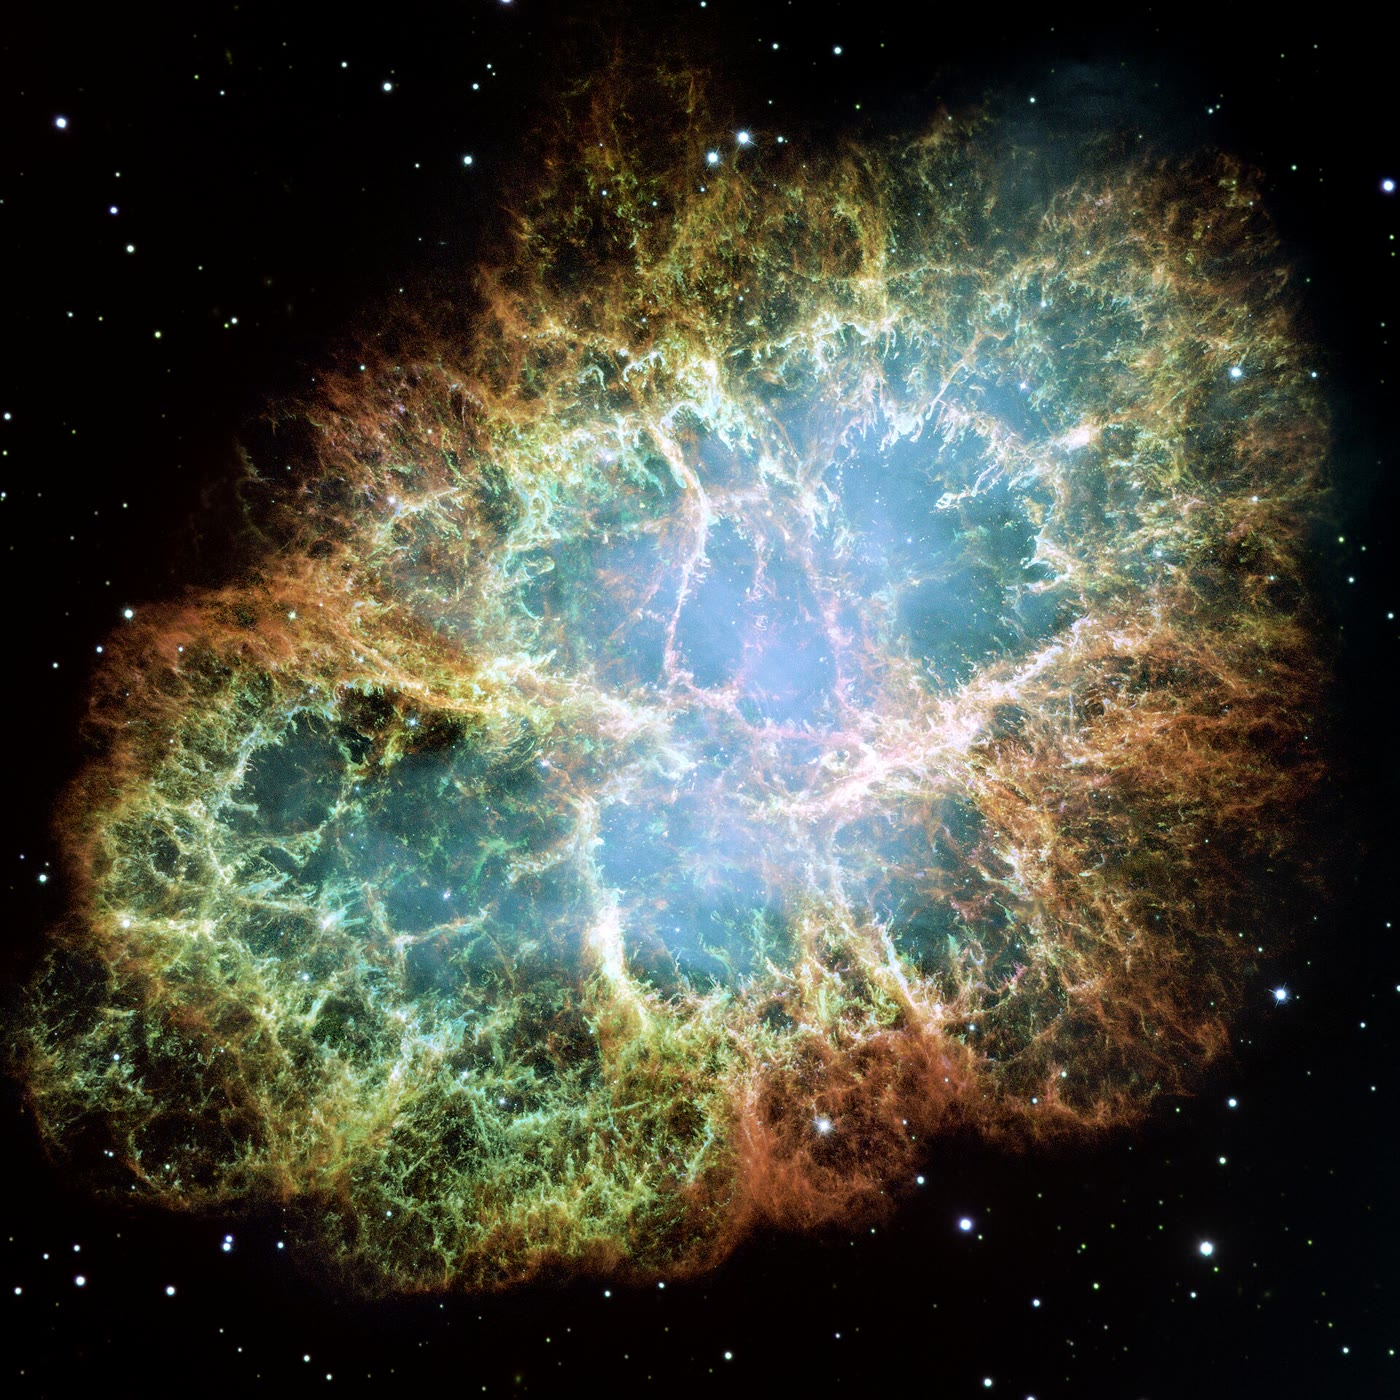
\includegraphics[width=0.5\linewidth]{images/book5/b3-crab-nebula.jpg}
\par\smallskip{\small Nebula Kepiting, mosaik 24 eksposur Teleskop Luar
Angkasa Hubble: sisa yang mengembang dari bintang yang ledakannya
dicatat astronom Jepang dan Tiongkok pada 1054. Filamen oranye
adalah lapisan luar bintang yang compang-camping, sebagian besar hidrogen; kilau
kebiruan di dalamnya berasal dari elektron yang berputar spiral di sekitar garis
medan magnet bintang neutron di pusat, yang berputar tiga puluh kali per
detik. Gas filamen, yang membawa apa yang dibentuk bintang, bercampur
ke dalam medium antarbintang. NASA, ESA, J.~Hester dan A.~Loll, domain
publik.}\label{fig:b3:origin-of-elements:crab}
\end{omfigure}
% ledger: photo:b3-crab-nebula

\section{Penangkapan neutron}\label{sec:b3:origin-of-elements:neutrons}

Neutron tidak bermuatan listrik dan tidak ditolak oleh inti: bahkan
neutron lambat pun masuk ke dalamnya, dan inti itu, yang massanya satu satuan lebih berat, melepaskan
energi ikatnya sebagai sinar gamma. Penangkapan berulang menghasilkan isotop yang lebih berat
dari unsur yang sama hingga salah satunya tidak stabil; ia kemudian meluruh,
biasanya lewat peluruhan beta-minus, menjadi unsur berikutnya, yang kemudian
menangkap neutron. Inti mana yang terbentuk bergantung pada satu perbandingan: waktu antara
dua penangkapan dibandingkan dengan waktu paruh inti tak stabil yang ditemui di
sepanjang jalan.

\begin{definition}[Penangkapan neutron; proses s; proses r]\label{def:b3:origin-of-elements:s-process}
Yang disebut \emph{penangkapan neutron}\index{penangkapan neutron} adalah penyerapan
neutron bebas oleh sebuah inti, $(Z, A) + \mathrm{n} \to (Z, A+1) + \gamma$.
Dalam \emph{proses s}\index{s-process@proses s} (lambat), penangkapan
lebih lambat daripada kebanyakan peluruhan beta: waktu antara dua penangkapan pada satu
inti adalah ratusan sampai ribuan tahun, sehingga inti tak stabil
hampir selalu meluruh sebelum sempat menangkap, dan rantai penangkapan
dan peluruhan mengikuti lembah kestabilan. Dalam
\emph{proses r}\index{r-process@proses r} (cepat), massa jenis neutron
sangat tinggi sehingga penangkapan jauh lebih cepat daripada peluruhan: inti-inti
didorong menjadi isotop yang sangat kaya neutron, jauh dari kestabilan, dalam beberapa
detik, dan meluruh kembali ke kestabilan begitu neutron habis.
\end{definition}
% ledger: cowan21:timescales, cowan21:rprocess, kaeppeler11:overview

Kedua proses mencapai inti yang berbeda, dan bagan nuklida
menunjukkan yang mana. Gambar di bawah menggambarkan sejalur bagan itu, mulai dari kadmium
sampai barium. \omterm{def:b3:origin-of-elements:s-process}{Proses s} menaiki bagan itu sepanjang lembah kestabilan: sepanjang satu
baris unsur selama isotop-isotopnya stabil, lalu naik satu baris oleh satu
peluruhan beta. \omterm{def:b3:origin-of-elements:s-process}{Proses r} berasal dari sisi kaya neutron, bagian kanan bawah:
setiap inti yang sangat kaya neutron meluruh berturut-turut lewat
peluruhan beta-minus sepanjang isobarnya, dengan mempertahankan nomor massanya, dan berhenti di
inti stabil pertama yang dijumpainya. Inti stabil yang punya isobar stabil dengan
$Z$ yang lebih rendah \emph{terlindung} dari \omterm{def:b3:origin-of-elements:s-process}{proses r}: $^{122}\mathrm{Te}$
berada di belakang $^{122}\mathrm{Sn}$, $^{123}\mathrm{Te}$ di belakang
$^{123}\mathrm{Sb}$, $^{124}\mathrm{Te}$ di belakang $^{124}\mathrm{Sn}$.
Ketiga inti ini hanya dapat dibentuk oleh \omterm{def:b3:origin-of-elements:s-process}{proses s}: mereka adalah
\emph{hanya-s}. Sebaliknya, $^{128}\mathrm{Te}$ dan $^{130}\mathrm{Te}$
berada di luar jalur s, sehingga telurium hanya tersisa pada $^{127}\mathrm{Te}$,
yang waktu paruhnya \qty{9.35}{h}: keduanya hanya-r.
% ledger: kaeppeler11:overview, data:b5-iaea-gs, data:b5-sigman

\begin{omfigure}
\centering
\begin{tikzpicture}
\begin{axis}[x=0.62cm, y=0.7cm, xmin=61.4, xmax=84.6, ymin=47.4, ymax=56.6,
  xlabel={nomor neutron $N$}, ylabel={},
  xtick={62,64,...,84}, ytick={48,...,56},
  yticklabels={Cd 48, In 49, Sn 50, Sb 51, Te 52, I 53, Xe 54, Cs 55, Ba 56},
  tick label style={font=\scriptsize}, label style={font=\small},
  axis line style={black!40}, clip=false,
  scatter/classes={0={mark=square*, mark size=6.5pt, blue!45},
    1={mark=square*, mark size=6.5pt, black!18},
    2={mark=square*, mark size=6.5pt, red!40},
    3={mark=square*, mark size=6.5pt, orange!45}}]
\addplot[only marks, mark=square, mark size=6.5pt, black!45, thin,
  restrict x to domain=61:85]
  table[x=N, y=Z] {figdata/out/bachelor-3-neutron_capture-unstable.dat};
\addplot[scatter, only marks, scatter src=explicit symbolic,
  restrict x to domain=61:85]
  table[x=N, y=Z, meta=cls] {figdata/out/bachelor-3-neutron_capture-chart.dat};
\addplot[only marks, mark=none, nodes near coords={\massnum},
  restrict x to domain=61:85,
  visualization depends on={value \thisrow{A} \as \massnum},
  nodes near coords align={center}, every node near coord/.append style={font=\tiny}]
  table[x=N, y=Z] {figdata/out/bachelor-3-neutron_capture-chart.dat};
\addplot[only marks, mark=none, nodes near coords={\massnum}, restrict x to domain=61:85,
  visualization depends on={value \thisrow{A} \as \massnum},
  nodes near coords align={center}, every node near coord/.append style={font=\tiny, black!55}]
  table[x=N, y=Z] {figdata/out/bachelor-3-neutron_capture-unstable.dat};
\addplot[quiver={u=0.48*\thisrow{dN}, v=0.48*\thisrow{dZ}}, -{Stealth[length=3pt]},
  blue!60!black, semithick, restrict x to domain=61:85]
  table[x expr=\thisrow{N0}+0.26*\thisrow{dN}, y expr=\thisrow{Z0}+0.26*\thisrow{dZ}]
  {figdata/out/bachelor-3-neutron_capture-path.dat};
\begin{scope}[red!70!black, dashed, -{Stealth[length=4pt]}, thick]
\draw (axis cs:79.1,48.9) -- (axis cs:76.4,51.6);
\draw (axis cs:81.1,48.9) -- (axis cs:78.4,51.6);
\draw (axis cs:83.1,50.9) -- (axis cs:80.4,53.6);
\end{scope}
\node[font=\scriptsize, red!70!black, anchor=south east, align=right] at (axis cs:84.5,47.5)
  {peluruhan proses r\\[-1pt]sepanjang isobar};
\end{axis}
\end{tikzpicture}
\par\smallskip{\small Sejalur bagan nuklida, dari kadmium
hingga barium, nomor neutron 62 sampai 84. Kotak berwarna adalah inti yang ditemukan di alam, diberi label
dengan nomor massanya: biru, hanya-s; abu-abu, dibentuk oleh kedua proses; merah,
hanya-r; oranye, \omterm{def:b3:origin-of-elements:p-process}{inti p}, tidak dicapai keduanya. Kotak terbuka adalah
inti tak stabil yang dilewati \omterm{def:b3:origin-of-elements:s-process}{proses s}. Panah biru: jalur s,
penangkapan ke kanan, peluruhan beta secara diagonal ke atas dan ke kiri (pada
$^{134}\mathrm{Cs}$ dan $^{135}\mathrm{Cs}$ jalur itu bercabang). Panah merah putus-putus
menunjukkan tiga dari rantai peluruhan \omterm{def:b3:origin-of-elements:s-process}{proses r}, yang berakhir di
$^{128}\mathrm{Te}$, $^{130}\mathrm{Te}$, dan $^{134}\mathrm{Xe}$. Kelas
dihitung dari isotop yang ditemukan di alam (Asplund,
Amarsi dan Grevesse, 2021) serta waktu paruh dan moda peluruhan pada
bagan nuklida IAEA.}\label{fig:b3:origin-of-elements:chart}
\end{omfigure}
% ledger: data:b5-sigman, data:b5-iaea-gs, data:b5-asplund21, kaeppeler11:branchings

Kelompok ketiga, kotak oranye, tidak dicapai oleh kedua proses ini:
isotop kaya proton seperti $^{112}\mathrm{Sn}$, $^{120}\mathrm{Te}$
atau $^{124}\mathrm{Xe}$.

\begin{definition}[inti p]\label{def:b3:origin-of-elements:p-process}
\emph{Inti p}\index{inti p} adalah isotop stabil di sisi kaya proton
dari lembah kestabilan, di luar puncak besi, yang
tidak dapat dibentuk oleh \omterm{def:b3:origin-of-elements:s-process}{proses s} maupun \omterm{def:b3:origin-of-elements:s-process}{proses r}: mereka terlindung
dari \omterm{def:b3:origin-of-elements:s-process}{proses r} oleh isobar stabil dengan $Z$ lebih kecil, dan berada di luar
jalur s. Inti p dikaitkan dengan proses p yang terpisah, yang kemungkinan terjadi dalam
ledakan supernova, dan dengan sedikit pengecualian kelimpahannya jauh lebih kecil daripada
kelimpahan isotop s dan r tetangga.
\end{definition}
% ledger: kaeppeler11:overview

Aturan yang membaca bagan itu, diterapkan pada seluruh 287 nuklida dari
tabel proto-Matahari di atas seng, menemukan 30 nuklida hanya-s, 29 nuklida hanya-r
dan 36 \omterm{def:b3:origin-of-elements:p-process}{inti p}. Salah satu \omterm{def:b3:origin-of-elements:p-process}{inti p} ini, $^{176}\mathrm{Hf}$, sebenarnya dicapai oleh
\omterm{def:b3:origin-of-elements:s-process}{proses s} melalui keadaan tereksitasi berumur panjang pada
$^{176}\mathrm{Lu}$ yang diabaikan oleh aturan sederhana itu; 35 sisanya adalah \omterm{def:b3:origin-of-elements:p-process}{inti p}
dalam literatur.
% ledger: data:b5-sigman, kaeppeler11:branchings

\omterm{def:b3:origin-of-elements:s-process}{Proses s} dapat diikuti secara kuantitatif, karena nuklidanya berada dekat kestabilan dan
penampang lintang penangkapannya dapat diukur. Dalam plasma bintang pada suhu $T$,
neutron berada dalam kesetimbangan termal, dan yang penting adalah
penampang lintang yang dirata-ratakan terhadap distribusi Maxwell--Boltzmann mereka,
$\langle\sigma\rangle$, yang dinyatakan untuk energi termal
$kT = \qty{30}{keV}$.
% ledger: kaeppeler11:classical

\begin{proposition}[Relasi $\sigma N$]\label{prop:b3:origin-of-elements:sigma-n}
\index{relasi sigma N@relasi $\sigma N$}
Pada suatu ruas jalur s tempat setiap nuklida stabil dan rapat
neutron $n_\mathrm{n}$ serta suhunya konstan, misalkan $N_A$ adalah kelimpahan
nuklida bernomor massa $A$ dan $\langle\sigma\rangle_A$ penampang lintang rata-ratanya.
Jika aliran neutron telah mencapai
keadaan tunak, maka
\[
\langle\sigma\rangle_{A-1} N_{A-1} = \langle\sigma\rangle_A N_A ,
\]
sehingga hasil kali $\sigma N$ sama untuk setiap nuklida pada
ruas itu.
\end{proposition}

\begin{proof}
Sebuah nuklida bermassa $A$ menangkap neutron dengan laju
$\lambda_A = n_\mathrm{n}\langle\sigma\rangle_A v_T$ per nuklida, dengan $v_T$
adalah laju termal rata-rata neutron. Nuklida ini terbentuk dari penangkapan pada
$A - 1$ dan musnah karena penangkapan pada dirinya sendiri, sehingga
$\mathrm{d}N_A/\mathrm{d}t = n_\mathrm{n} v_T\,(\langle\sigma\rangle_{A-1}
N_{A-1} - \langle\sigma\rangle_A N_A)$. Dalam keadaan tunak turunannya
nol, dan itulah relasinya. Nuklida dengan penampang lintang besar
cepat diteruskan dan tetap jarang; yang berpenampang lintang kecil
menumpuk.
\end{proof}
% ledger: kaeppeler11:classical

Tiga isotop hanya-s dari telurium menguji relasi ini. Kelimpahan proto-Matahari mereka
adalah \num{0.1067}, \num{0.0373} dan \num{0.1984} atom per
satu juta atom silikon, dan penampang lintangnya \num{295}, \num{832} dan
\qty{155}{mb}: hasil kalinya \num{31.5}, \num{31.0} dan
\qty{30.8}{mb}, sama dalam tiga persen, meskipun kelimpahannya
berbeda sekitar lima kali. Melintasi bilangan ajaib neutron, relasi ini
patah: nuklida dengan $N = 50$, $82$ atau $126$ terikat sangat erat
sehingga sulit menangkap neutron, $\langle\sigma\rangle = \qty{4.0}{mb}$ untuk
$^{138}\mathrm{Ba}$ dibandingkan \qty{61.2}{mb} untuk $^{136}\mathrm{Ba}$, dan
mereka berperan sebagai sumbatan. Gambar di bawah menunjukkan hasil kali untuk
semua nuklida hanya-s: dataran datar yang dipisahkan oleh lompatan di dekat
$A = 88$, $140$ dan $208$.
% ledger: data:b5-sigman, data:b5-kadonis, kaeppeler11:classical

\begin{omfigure}
\centering
\begin{tikzpicture}
\begin{axis}[width=0.95\linewidth, height=7.4cm, xmin=60, xmax=212,
  ymode=log, ymin=1, ymax=5000, xlabel={nomor massa $A$},
  ylabel={$\langle\sigma\rangle N$ (mb, per $10^6$ atom Si)},
  tick label style={font=\scriptsize}, label style={font=\small},
  legend style={font=\scriptsize, at={(0.5,-0.17)}, anchor=north,
    legend columns=2, draw=none, cells={anchor=west},
    /tikz/every even column/.append style={column sep=1em}}]
\draw[black!35, dotted, thick] (axis cs:88,1) -- (axis cs:88,5000);
\draw[black!35, dotted, thick] (axis cs:139,1) -- (axis cs:139,5000);
\draw[black!35, dotted, thick] (axis cs:208,1) -- (axis cs:208,5000);
\addplot[blue!70!black, thick, const plot]
  table[x=A, y=sigN_model] {figdata/out/bachelor-3-neutron_capture-fitted.dat};
\addlegendentry{model klasik dicocokkan untuk $A > 90$}
\addplot[only marks, mark=*, mark size=1.7pt, red!70!black]
  table[x=A, y=sigN] {figdata/out/bachelor-3-neutron_capture-sigman.dat};
\addlegendentry{nuklida hanya-s}
\begin{scope}[font=\scriptsize]
\node[anchor=south west] at (axis cs:88.5,1.1) {$N = 50$};
\node[anchor=south west] at (axis cs:139.5,1.1) {$N = 82$};
\node[anchor=south east] at (axis cs:207.5,1.1) {$N = 126$};
\node[anchor=south] at (axis cs:123,38) {Te};
\node[anchor=south] at (axis cs:135,33) {Ba};
\node[anchor=north] at (axis cs:149,6.6) {Sm};
\node[anchor=west] at (axis cs:177,1.79) {Lu};
\node[anchor=west] at (axis cs:71,2326) {Ge};
\node[anchor=west] at (axis cs:83,428) {Kr};
\end{scope}
\end{axis}
\end{tikzpicture}
\par\smallskip{\small Hasil kali penampang lintang \omterm{def:b3:origin-of-elements:s-process}{penangkapan neutron}
pada \qty{30}{keV} (KADoNiS) dan kelimpahan proto-Matahari (Asplund,
Amarsi dan Grevesse, 2021) untuk 30 nuklida hanya-s. Di antara bilangan ajaib
neutron (garis putus-putus) hasil kali ini hampir konstan; pada setiap
bilangan ajaib aliran dihambat dan hasil kalinya turun. Garis itu adalah model klasik
\omterm{def:b3:origin-of-elements:s-process}{proses s} yang dicocokkan di sini terhadap nuklida yang lebih berat dari $A = 90$.
Nuklida yang lebih ringan memerlukan komponen kedua yang lebih lemah,
dibentuk dalam bintang masif.}\label{fig:b3:origin-of-elements:sigma-n}
\end{omfigure}
% ledger: data:b5-sigman, data:b5-kadonis, data:b5-asplund21, kaeppeler11:classical

Garis pada gambar adalah model klasik \omterm{def:b3:origin-of-elements:s-process}{proses s}: sebagian kecil $G$ dari besi-56
terpapar neutron, dengan paparan tersebar secara eksponensial di sekitar
rata-rata $\tau_0$, dan aliran diikuti nuklida demi nuklida dengan
penampang lintang yang terukur. Kecocokannya pada 22 nuklida hanya-s
yang lebih berat dari $A = 90$ (tidak termasuk $^{176}\mathrm{Lu}$, yang
meluruh, dan $^{187}\mathrm{Os}$, yang diberi makan oleh peluruhan
$^{187}\mathrm{Re}$) memberikan $\tau_0 = \qty{0.31}{mb^{-1}}$ dan
$G = \qty{0.054}{\percent}$ dari besi-56 Matahari, mendekati
\qty{0.04}{\percent} dari analisis terperinci, yang menyatakan bahwa setiap
nuklida benih rata-rata menangkap sekitar lima belas neutron. Nuklida hanya-s
teringan, germanium-70 dan selenium-76, berada jauh di atas garis: keduanya
memerlukan komponen kedua yang lemah, dibentuk dalam bintang masif.
% ledger: data:b5-sigman, kaeppeler11:classical

Apabila nuklida tak stabil pada lintasan hidup kira-kira sama lamanya dengan waktu
antara dua penangkapan, aliran terbagi: sebagian meluruh, sebagian menangkap.
Yang disebut \emph{percabangan} terjadi pada $^{79}\mathrm{Se}$, $^{85}\mathrm{Kr}$,
$^{134}\mathrm{Cs}$, $^{147}\mathrm{Pm}$, dan $^{151}\mathrm{Sm}$, antara
lain. Percabangan memungkinkan sebagian aliran melewati suatu nuklida: dari dua
isotop hanya-s samarium, $^{150}\mathrm{Sm}$ menerima seluruh
aliran dan $^{148}\mathrm{Sm}$ hanya bagian yang melewati
percabangan pada massa 147, dan rasio $\sigma N$ keduanya, \num{0.87},
mengukur pembagian itu. Karena pembagian ini bergantung pada kerapatan neutron dan
suhu, percabangan adalah termometer dan densimeter bagi
bintang tempat \omterm{def:b3:origin-of-elements:s-process}{proses s} berlangsung.
% ledger: kaeppeler11:branchings, kaeppeler11:pairs, data:b5-sigman

\begin{inthelab}[Mengukur penampang lintang penangkapan]
Untuk mengukur penampang lintang rata-rata yang dibutuhkan \omterm{def:b3:origin-of-elements:s-process}{proses s},
para fisikawan mereproduksi spektrum neutron bintang di akselerator.
Proton yang menumbuk target litium menghasilkan neutron melalui reaksi
$^{7}\mathrm{Li}(\mathrm{p},\mathrm{n})^{7}\mathrm{Be}$, yang spektrumnya
meniru spektrum termal pada $kT = \qty{25}{keV}$, mendekati
\qty{23}{keV} kilatan lapisan helium raksasa merah. Sampel diletakkan
tepat di samping target, pada fluks terkuat, dan setelah
iradiasi, sinar gamma dari nuklida radioaktif yang baru dibuat
dihitung: metode aktivasi ini bekerja dengan sampel kurang dari
satu mikrogram. Jika produknya stabil, neutron dikirim dalam denyut
dan diukur waktunya selama lintasan terbang untuk menentukan energinya, dan bola
kristal barium fluorida di sekeliling sampel mencatat
kaskade sinar gamma pada setiap penangkapan.
\end{inthelab}
% ledger: kaeppeler11:lab

\begin{history}[Teknesium pada raksasa merah]
Pada 1952 P.~W.~Merrill menemukan garis teknesium dalam spektrum
raksasa merah tipe spektral S. Teknesium tidak memiliki isotop stabil; yang
dibuat oleh \omterm{def:b3:origin-of-elements:s-process}{proses s}, $^{99}\mathrm{Tc}$, memiliki waktu paruh
\num{211000} tahun, jauh lebih pendek daripada masa hidup yang
telah dijalani bintang-bintang ini. Teknesium harus dibuat di dalam bintang, dan
baru-baru ini. Itulah bukti langsung pertama bahwa bintang membentuk unsur.
Pada 1957 E.~M. dan G.~R.~Burbidge, W.~A.~Fowler dan F.~Hoyle, serta
secara independen A.~G.~W.~Cameron, merumuskan model klasik
\omterm{def:b3:origin-of-elements:s-process}{proses s}.
\end{history}
% ledger: kaeppeler11:overview, data:b5-iaea-gs

\omterm{def:b3:origin-of-elements:s-process}{Proses r} meninggalkan puncaknya sendiri. Lintasannya berada dekat dengan garis tetes neutron,
yaitu batas di luar mana nuklida tidak dapat menahan neutron tambahan,
dan aliran menunggu pada nuklida dengan kulit neutron tertutup, $N = 50$, $82$ dan
$126$, sampai nuklida itu meluruh beta. Titik-titik tunggu ini menumpuk materi;
setelah peluruhan akhir menuju kestabilan, tumpukan itu berada pada nomor massa beberapa
satuan lebih rendah daripada puncak \omterm{def:b3:origin-of-elements:s-process}{proses s} pada bilangan ajaib yang sama, yang
terbentuk dari nuklida stabil: sekitar $A = 130$ (telurium dan xenon) dan
$A = 195$ (platina), dibandingkan $A = 138$ dan $208$ untuk puncak s
barium dan timbal. Kurva kelimpahan memperlihatkan kedua kelompok puncak berdampingan
satu sama lain. \omterm{def:b3:origin-of-elements:s-process}{Proses r} menghasilkan sekitar separuh unsur berat, \omterm{def:b3:origin-of-elements:s-process}{proses s}
separuh sisanya.
% ledger: cowan21:rprocess, kaeppeler11:overview, kaeppeler11:classical

\section{Tempat proses berlangsung}\label{sec:b3:origin-of-elements:sites}

\omterm{def:b3:origin-of-elements:s-process}{Proses s} utama berlangsung di raksasa merah dengan massa hingga sekitar tiga massa Matahari, dekat
akhir hidupnya, sebagai bintang cabang raksasa asimtotik. Di antara kilatan
pembakaran helium pada kulit di sekitar inti mereka, lapisan tipis kaya
karbon-13 terbentuk; pada sekitar \qty{9e7}{K} reaksi
$^{13}\mathrm{C}(\alpha,\mathrm{n})^{16}\mathrm{O}$ melepaskan neutron
selama sekitar sepuluh ribu tahun, pada kerapatan $10^6$ sampai
\num{e8}\text{ neutron}\,\unit{cm^{-3}}. Selama kilatan itu sendiri, di atas
\qty{2.5e8}{K}, $^{22}\mathrm{Ne}(\alpha,\mathrm{n})^{25}\mathrm{Mg}$
menghasilkan semburan selama beberapa tahun pada kerapatan hingga \qty{e10}{cm^{-3}}. Produknya
dibawa naik ke permukaan, tempat teknesium teramati, dan terhempas
oleh angin bintang. \omterm{def:b3:origin-of-elements:s-process}{Proses s} lemah, yang membentuk nuklida hanya-s
yang lebih ringan dari $A = 90$, berlangsung di bintang masif selama pembakaran helium dan
pembakaran karbon mereka.
% ledger: kaeppeler11:sources, kaeppeler11:overview

Supernova keruntuhan inti, akhir hidup bintang di atas delapan hingga sepuluh
massa Matahari, mengembalikan \omterm{def:b3:origin-of-elements:alpha}{unsur alfa} dan sebagian besi segera setelah
kelahiran bintang, karena bintang masif berumur pendek. Supernova tipe~Ia,
yaitu katai putih yang meledak dalam sistem biner, mengembalikan sebagian besar
besi, tetapi hanya setelah jeda: katai putih harus terbentuk lebih dulu, dari
bintang bermassa kurang dari delapan massa Matahari, lalu entah mengumpulkan materi dari
pendampingnya hingga mencapai massa Chandrasekhar, sekitar
\qty{1.44}{M_\odot}, atau bergabung dengan katai putih kedua. \omterm{def:b3:origin-of-elements:s-process}{Proses r} memerlukan
tempat yang jauh lebih ekstrem.
% ledger: matteucci21:production, matteucci21:time-delay

\begin{definition}[Penggabungan bintang neutron; kilonova]\label{def:b3:origin-of-elements:kilonova}
Yang disebut \emph{penggabungan bintang neutron}\index{penggabungan bintang neutron} adalah
penyatuan dua bintang neutron dalam sistem biner rapat, yang orbitnya telah
menyusut akibat pemancaran gelombang gravitasi. Sebagian materi kaya neutron
terlempar keluar. Yang disebut \emph{kilonova}\index{kilonova} adalah pendaran sesaat
dari ejekta itu, yang dipanaskan oleh peluruhan radioaktif nuklida
\omterm{def:b3:origin-of-elements:s-process}{proses r} yang baru terbentuk, dan berlangsung berhari-hari.
\end{definition}
% ledger: cowan21:kilonova, ligo17:gw170817

Pada 17 Agustus 2017 detektor gelombang gravitasi merekam
spiral mendekat dua bintang neutron, GW170817, pada jarak sekitar
\qty{40}{Mpc}: dua benda bermassa \num{1.17} hingga \qty{1.60}{M_\odot}, bersama-sama
\qty{2.74}{M_\odot}. Semburan sinar gamma tiba \qty{1.7}{s} setelah
penggabungan. Kurang dari sebelas jam kemudian teleskop menemukan titik cahaya baru
di galaksi NGC~4993 (gambar di bawah). Pendaran ultravioletnya memudar
dalam dua hari, dan selama sepuluh hari cahayanya berubah menjadi merah dan inframerah.
Model evolusi itu memerlukan beberapa komponen ejekta, yang
paling merah kaya lantanida, yakni unsur berat \omterm{def:b3:origin-of-elements:s-process}{proses r} yang
hutan garisnya yang rapat membuat ejekta buram. Taksiran massa total ejekta
yang terlempar adalah \num{0.03} hingga \qty{0.08}{M_\odot}: bukti langsung pertama
bahwa \omterm{def:b3:origin-of-elements:kilonova}{penggabungan bintang neutron} membentuk unsur \omterm{def:b3:origin-of-elements:s-process}{proses r}.
% ledger: ligo17:gw170817, mma17:kilonova, cowan21:kilonova

\begin{omfigure}
\centering
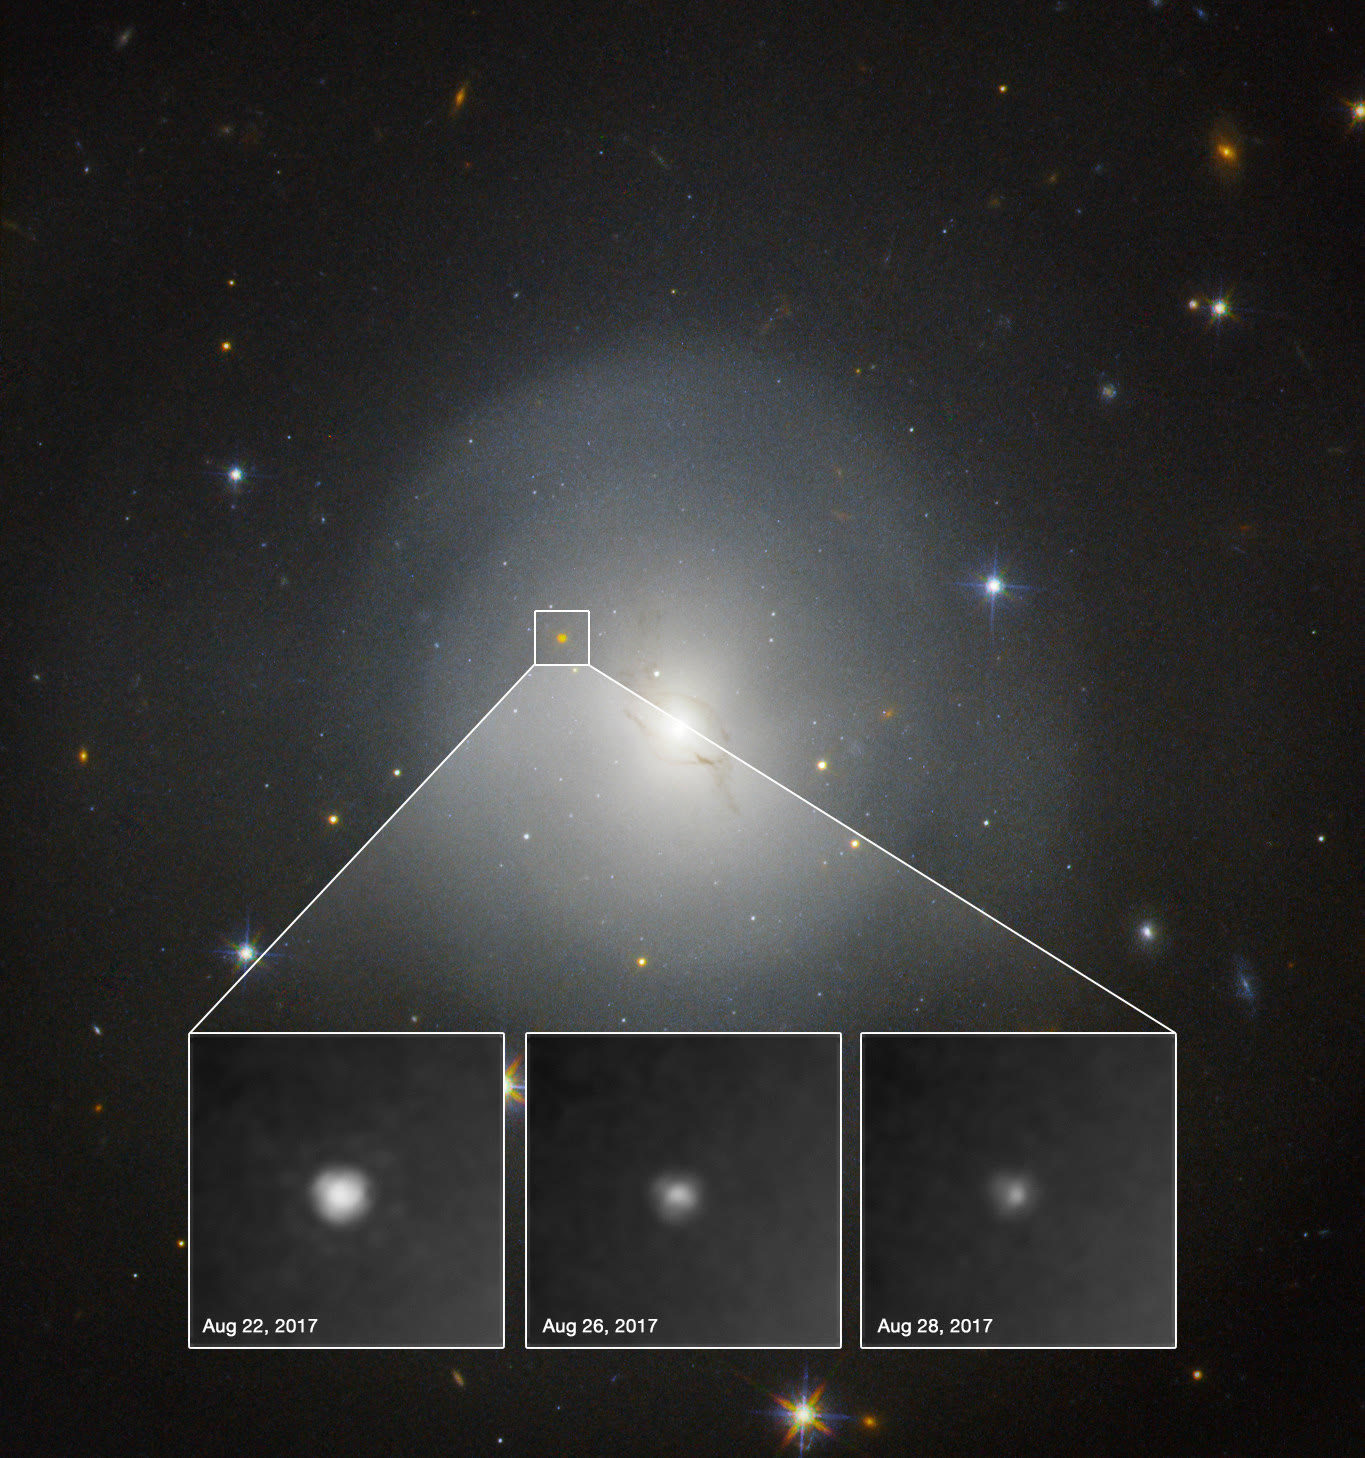
\includegraphics[width=0.55\linewidth]{images/book5/b3-kilonova.jpg}
\par\smallskip{\small Galaksi NGC~4993 difoto oleh Teleskop Luar Angkasa Hubble
setelah penggabungan dua bintang neutron yang terdeteksi lewat
gelombang gravitasi pada 17 Agustus 2017. Kotak menandai \omterm{def:b3:origin-of-elements:kilonova}{kilonova}; sisipan,
yang diambil pada 22, 26 dan 28 Agustus, memperlihatkannya meredup selama enam hari.
NASA dan ESA (A.~J.~Levan, N.~R.~Tanvir, A.~Fruchter dan O.~Fox), CC
BY~4.0.}\label{fig:b3:origin-of-elements:kilonova}
\end{omfigure}
% ledger: photo:b3-kilonova

\begin{dated}{2021}
Apakah \omterm{def:b3:origin-of-elements:kilonova}{penggabungan bintang neutron} menghasilkan sebagian besar unsur
r-proses di Galaksi belum terjawab. Penggabungan menunggu orbit biner
mereka meluruh, dan model evolusi Galaksi yang menjadikannya satu-satunya
sumber menghasilkan unsur r-proses terlalu lambat untuk menjelaskan apa yang
teramati pada bintang-bintang paling tua dan paling miskin logam. Jenis supernova
keruntuhan inti yang langka, dengan rotasi cepat dan medan magnet kuat, serta keruntuhan
bintang-bintang sangat masif menjadi kandidat lain; satu model Galaksi
menjelaskan europium yang teramati jika sekitar tiga persen dari
hipernova bermassa 25 hingga \qty{50}{M_\odot} adalah jenis yang
didorong medan magnet.
\end{dated}
% ledger: kobayashi20:origins, cowan21:rprocess

\section{Evolusi kimia Galaksi}\label{sec:b3:origin-of-elements:gce}

Setiap generasi bintang mengembalikan ke gas sebagian dari yang telah dibuatnya,
dan generasi berikutnya terbentuk dari gas yang diperkaya itu. Komposisi
sebuah bintang karena itu mencatat komposisi gas saat kelahirannya, dan
bintang-bintang dalam sebuah galaksi, jika diurutkan menurut umur, mencatat sejarahnya.

\begin{definition}[Evolusi kimia Galaksi]\label{def:b3:origin-of-elements:gce}
Yang disebut \emph{evolusi kimia Galaksi}\index{evolusi kimia Galaksi}
adalah perubahan komposisi gas dan bintang di sebuah galaksi terhadap waktu,
di bawah aksi gabungan pembentukan bintang, \omterm{def:b3:origin-of-elements:yield}{hasil bintang}, umur bintang, dan gas
yang masuk ke dalam galaksi atau terdorong keluar darinya; serta kajian
perubahan itu dengan model yang dibandingkan dengan kelimpahan bintang
berumur diketahui.
\end{definition}
% ledger: matteucci21:simple

Model paling sederhana memperlakukan suatu wilayah galaksi sebagai satu kotak
gas yang tercampur baik dan perlahan berubah menjadi bintang. Misalkan $s$
massa yang terkunci dalam bintang berumur panjang dan sisa bintang,
$M_\mathrm{g}$ massa gas, dan $M = M_\mathrm{g} + s$ total massanya. \emph{Hasil
per generasi bintang} $y$ adalah massa logam baru yang dikembalikan suatu
generasi bintang ke gas per satuan massa yang dikuncinya.
% ledger: matteucci21:yield

\begin{theorem}[Model kotak tertutup]\label{thm:b3:origin-of-elements:closed-box}
\index{model kotak tertutup}
Tinjau suatu wilayah yang tidak bertukar gas dengan sekelilingnya, mulai
sebagai gas murni tanpa logam, tetap tercampur baik, dan bintang-bintang
yang membuat logam mati seketika sementara yang lain hidup selamanya
(daur ulang seketika). Maka \omterm{def:b3:origin-of-elements:metallicity}{metalisitas} gas adalah
\[
Z = y \ln\frac{1}{\mu}, \qquad \mu = \frac{M_\mathrm{g}}{M},
\]
dengan $\mu$ adalah fraksi gas, dan massa bintang yang terbentuk dengan
\omterm{def:b3:origin-of-elements:metallicity}{metalisitas} di bawah $Z$ adalah \mbox{$M\,(1 - \mathrm{e}^{-Z/y})$}.
\end{theorem}

\begin{proof}
Ketika massa $\mathrm{d}s$ terkunci ke dalam bintang, gas kehilangan
$\mathrm{d}s$ beserta logam yang dikandungnya, $Z\,\mathrm{d}s$,
dan memperoleh $y\,\mathrm{d}s$ logam baru:
$\mathrm{d}M_\mathrm{g} = -\mathrm{d}s$ dan
$\mathrm{d}(Z M_\mathrm{g}) = (y - Z)\,\mathrm{d}s$. Menjabarkan
yang kedua, $M_\mathrm{g}\,\mathrm{d}Z + Z\,\mathrm{d}M_\mathrm{g} =
y\,\mathrm{d}s - Z\,\mathrm{d}s$, dan suku-suku dalam $Z$ saling meniadakan:
$M_\mathrm{g}\,\mathrm{d}Z = -y\,\mathrm{d}M_\mathrm{g}$. Mengintegralkan
dari $M_\mathrm{g} = M$, $Z = 0$ menghasilkan $Z = y\ln(M/M_\mathrm{g})$. Bintang
yang terbentuk ketika \omterm{def:b3:origin-of-elements:metallicity}{metalisitas} gas berada di bawah $Z$ adalah bintang yang
terbentuk ketika gas turun dari $M$ ke $M\mathrm{e}^{-Z/y}$, yakni sebesar
$M(1 - \mathrm{e}^{-Z/y})$.
\end{proof}
% ledger: matteucci21:simple

Model ini memprediksi distribusi \omterm{def:b3:origin-of-elements:metallicity}{metalisitas} bintang berumur panjang.
Di lingkungan Matahari, massa jenis permukaan gas adalah
\qty{13.7}{M_\odot.pc^{-2}} dan massa jenis bintang serta sisa bintang
\qty{33.4}{M_\odot.pc^{-2}}, sehingga $\mu = 13.7/47.1 = 0.29$. Jika gas saat
ini memiliki $Z = 0.0154$ seperti Matahari purba, hasilnya
adalah $y = 0.0154/\ln(1/0.29) = 0.0125$, dan fraksi dari seluruh bintang yang
terbentuk sejauh ini yang memiliki $Z$ di bawah sepersepuluh nilai sekarang,
$[\mathrm{Fe/H}] < -1$ jika besi mengikuti logam, adalah
$(1 - 0.29^{0.1})/(1 - 0.29) = 0.16$.
% ledger: mckee15:surface, asplund21:xyz, data:b5-gce

\begin{omfigure}
\centering
\begin{tikzpicture}
\begin{axis}[width=0.95\linewidth, height=7.2cm, xmin=-1.6, xmax=0.7,
  ymin=0, ymax=1500, xlabel={$[\mathrm{Fe/H}]$},
  ylabel={jumlah bintang per \num{0.1}~dex},
  tick label style={font=\scriptsize}, label style={font=\small},
  legend style={font=\scriptsize, at={(0.5,-0.17)}, anchor=north,
    legend columns=3, draw=none, cells={anchor=west},
    /tikz/every even column/.append style={column sep=1em}}]
\addplot[ybar, area legend, bar width=0.085, fill=black!25, draw=black!50, bar shift=0pt]
  table[x=feh, y=n_obs] {figdata/out/bachelor-3-chemical_evolution-mdf.dat};
\addlegendentry{katai F dan G (6670)}
\addplot[ybar, area legend, bar width=0.085, fill=blue!55, draw=blue!70!black, bar shift=0pt]
  table[x=feh, y=n_low] {figdata/out/bachelor-3-chemical_evolution-mdf.dat};
\addlegendentry{paling banyak \qty{1}{M_\odot} (902)}
\addplot[red!75!black, very thick, const plot mark mid]
  table[x=feh, y=model] {figdata/out/bachelor-3-chemical_evolution-mdf.dat};
\addlegendentry{kotak tertutup}
\draw[black!50, dashed] (axis cs:-1,0) -- (axis cs:-1,1500);
\node[font=\scriptsize, anchor=north west, align=left] at (axis cs:-1.57,1450)
  {kotak tertutup: \qty{16}{\percent}\\di bawah $-1$;\\teramati: \qty{0.4}{\percent}};
\end{axis}
\end{tikzpicture}
\par\smallskip{\small \omterm{def:b3:origin-of-elements:g-dwarf}{Masalah katai G}. Batang: \omterm{def:b3:origin-of-elements:metallicity}{metalisitas}
katai F dan G di lingkungan Matahari (Geneva--Copenhagen
survei, sampel fotometri terbaik yang dianalisis ulang oleh Casagrande dan rekan-rekan,
2011), semua bintang dalam abu-abu, dan yang bermassa paling banyak satu massa Matahari, bintang
berumur panjang yang dihitung model, dalam biru. Garis: kotak tertutup
dengan fraksi gas saat ini di lingkungan Matahari, diskalakan ke
jumlah bintang yang sama; model ini tidak menghasilkan bintang yang lebih kaya
daripada gas sekarang, yang dianggap bermetalisitas Matahari. Kotak ini memprediksi ekor panjang bintang miskin
logam yang tidak ada.}\label{fig:b3:origin-of-elements:g-dwarf}
\end{omfigure}
% ledger: data:b5-gcs, casagrande11:gcs, data:b5-gce, mckee15:surface

\begin{definition}[Masalah katai G]\label{def:b3:origin-of-elements:g-dwarf}
Yang disebut \emph{masalah katai G}\index{masalah katai G} adalah kekurangan
bintang berumur panjang yang miskin logam di lingkungan Matahari dibandingkan dengan
prediksi \omterm{thm:b3:origin-of-elements:closed-box}{model kotak tertutup}: jauh lebih sedikit katai berumur panjang
bertipe spektral G yang bermetalisitas rendah daripada yang seharusnya
dihasilkan kotak tertutup.
\end{definition}
% ledger: matteucci21:simple

Dari 6670 bintang dalam sampel survei, 26 memiliki $[\mathrm{Fe/H}] < -1$:
\qty{0.4}{\percent}, dibandingkan dengan \qty{16}{\percent} pada kotak tertutup.
Bahkan di antara 902 bintang dengan massa paling besar satu massa Matahari,
perbandingan yang paling adil, 26 bintang itu membentuk \qty{2.9}{\percent}. Jalan keluarnya adalah membuka
kotak itu: jika cakram di lingkungan Matahari dibentuk oleh aliran masuk lambat
gas miskin logam selama beberapa miliar tahun, gas awal tidak pernah
menjadi reservoir besar yang menunggu untuk membentuk bintang miskin logam, dan ekor
lenyap. Model cakram yang mereproduksi distribusi memerlukan waktu aliran masuk
lebih panjang daripada tiga sampai empat miliar tahun.
% ledger: data:b5-gcs, data:b5-gce, matteucci21:simple

Jam kedua adalah rasio dua jenis unsur. \omterm{def:b3:origin-of-elements:alpha}{Unsur alfa}
berasal dari supernova keruntuhan inti, segera setelah suatu generasi
bintang lahir; sebagian besar besi berasal dari supernova Tipe~Ia;
jauh setelahnya. Pada bintang halo tua, dengan $[\mathrm{Fe/H}] < -1$,
$[\alpha/\mathrm{Fe}]$ sekitar $+0.4$: bintang-bintang ini terbentuk dari gas
yang diperkaya oleh supernova keruntuhan inti saja. Pada bintang cakram, nilainya turun
seiring naiknya \omterm{def:b3:origin-of-elements:metallicity}{metalisitas} hingga nol, nilai Matahari, ketika supernova Tipe~Ia
menambahkan besinya. Gambar berikut menunjukkan model paling sederhana
dari gambaran \emph{penundaan waktu} ini: dalam kotak tertutup, kedua jenis
supernova mulai bersamaan, kecuali bahwa supernova Tipe~Ia dimulai dengan tenggang waktu tetap
sejak bintang-bintang pertama.
% ledger: matteucci21:time-delay, matteucci21:production

\begin{omfigure}
\centering
\begin{tikzpicture}
\begin{axis}[width=0.8\linewidth, height=6.4cm, xmin=-2.4, xmax=0.25,
  ymin=-0.08, ymax=0.55, xlabel={$[\mathrm{Fe/H}]$},
  ylabel={$[\alpha/\mathrm{Fe}]$},
  tick label style={font=\scriptsize}, label style={font=\small}]
\addplot[black!40, dashed, domain=-2.4:0.25, samples=2] {0};
\addplot[blue!70!black, very thick]
  table[x=feh, y=afe] {figdata/out/bachelor-3-chemical_evolution-alpha.dat};
\addplot[only marks, mark=*, mark size=2pt, red!70!black] coordinates {(-1,0.4) (0,0)};
\node[font=\scriptsize, anchor=south, align=center] at (axis cs:-1.75,0.41)
  {supernova keruntuhan inti saja};
\node[font=\scriptsize, anchor=south west, align=left] at (axis cs:-0.98,0.41)
  {supernova Tipe Ia\\[-1pt]mulai};
\node[font=\scriptsize, anchor=south west] at (axis cs:0.01,0.01) {Matahari};
\end{axis}
\end{tikzpicture}
\par\smallskip{\small Model dua fase $[\alpha/\mathrm{Fe}]$ dalam
kotak tertutup: dataran pada $+0.4$ adalah rasio yang dihasilkan supernova keruntuhan inti;
supernova Tipe~Ia, yang mulai ketika gas telah mencapai
$[\mathrm{Fe/H}] = -1$, kemudian menambahkan besi dengan laju tetap, hingga rasionya
sama dengan Matahari pada $[\mathrm{Fe/H}] = 0$. Dataran dan lututnya adalah yang
terlihat pada bintang-bintang Galaksi; bentuk di antaranya adalah milik model.
Pada \omterm{def:b3:origin-of-elements:metallicity}{metalisitas} Matahari, \qty{60}{\percent} besi dalam model ini
berasal dari supernova Tipe~Ia.}\label{fig:b3:origin-of-elements:alpha}
\end{omfigure}
% ledger: data:b5-gce, matteucci21:time-delay

Model rinci Galaksi yang mereproduksi tren yang teramati
mengambil dua pertiga besi dari supernova Tipe~Ia dan sepertiga dari
supernova keruntuhan inti, serta mendapati bahwa gas Galaksi muda
mencapai $[\mathrm{Fe/H}] = -1$ dalam sekitar satu sampai satu setengah miliar
tahun. Rasio ini adalah jam: populasi yang kaya \omterm{def:b3:origin-of-elements:alpha}{unsur alfa}
pada \omterm{def:b3:origin-of-elements:metallicity}{metalisitas} tertentu membentuk bintangnya dengan cepat, sebelum
supernova Tipe~Ia sempat menambahkan besinya. \omterm{def:b3:milky-way-galaxies:structure}{Cakram tebal} pada bab sebelumnya
adalah populasi seperti itu: tua, dan sedikit lebih kaya \omterm{def:b3:origin-of-elements:alpha}{unsur alfa}
dibandingkan bintang cakram tipis dengan \omterm{def:b3:origin-of-elements:metallicity}{metalisitas} yang sama.
% ledger: matteucci21:time-delay, casagrande11:gcs

\section{Dari kelimpahan Matahari ke Bumi}\label{sec:b3:origin-of-elements:earth}

Bumi terbuat dari bahan yang sama dengan Matahari, tetapi tidak dari seluruhnya.
Dalam nebula yang mendingin, hanya unsur yang mengembun menjadi padatan
yang dapat dikumpulkan menjadi planetesimal; volume Tahun~2 mengikuti
urutan saat unsur-unsur itu mengembun. Besi mengembun sebagai logam pada suhu yang kurang lebih
sama dengan silikat magnesium, \qtyrange{1310}{1340}{K} pada
\qty{e-4}{bar}, sehingga planet batuan mempertahankan bagian besinya, sedangkan
hidrogen, helium, karbon, nitrogen, dan gas mulia tetap berada di gas.
Dari gas dengan komposisi Matahari, hanya sekitar setengah persen massanya
yang mengembun menjadi batuan dan logam.
% ledger: lodders:tc-table, lodders:condensates

\begin{definition}[Tren volatilitas]\label{def:b3:origin-of-elements:volatility}
Yang disebut \emph{tren volatilitas}\index{tren volatilitas} suatu benda planet
adalah penurunan kelimpahannya, relatif terhadap kondrit CI dan
dinormalisasi ke suatu unsur refraktori, seiring menurunnya suhu kondensasi:
unsur refraktori berada pada proporsi kondritnya, sedangkan unsur agak volatil
berkurang makin banyak makin rendah
suhu kondensasinya.
\end{definition}

Untuk Bumi silikat, volume Tahun~2 menggambarkan tren terhadap
suhu kondensasi. Dinormalisasi ke magnesium, zirkonium
(mengembun pada \qty{1741}{K}) berada pada \num{1.11} kali
proporsi CI-nya; natrium (\qty{958}{K}) pada \num{0.22}, kalium
(\qty{1006}{K}) pada \num{0.19}, rubidium (\qty{800}{K}) pada \num{0.12}
dan seng (\qty{726}{K}) pada \num{0.075}. Bumi terbentuk dari material
yang sudah kehilangan sebagian unsur agak volatilnya sebelum
planet itu dirakit, atau kehilangannya selama pertumbuhannya. Bahkan kondrit CI
berbeda dari Matahari dengan cara yang mengikuti suhu kondensasi,
meskipun samar: unsur agak volatilnya berada
sekitar \num{0.04}~\omterm{def:b3:origin-of-elements:abundance}{dex} lebih tinggi daripada nilai fotosfer.
% ledger: lodders:tc-table, lodders:ci-table, ms95:pm-trace, asplund21:abstract

Jadi rekam jejak bab ini berlanjut hingga ke planet. Oksigen,
magnesium, dan silikon pada mantel adalah \omterm{def:b3:origin-of-elements:alpha}{unsur alfa} dari bintang masif;
besi pada inti sebagian besar berasal dari supernova Tipe~Ia;
torium dan uranium yang peluruhannya membantu memanaskan interior terletak di luar
bismut, tempat hanya \omterm{def:b3:origin-of-elements:s-process}{proses r} yang mencapai; dan seluruh campuran
disortir menurut volatilitas sebelum Bumi mengumpulkannya.
% ledger: matteucci21:production, matteucci21:time-delay, kaeppeler11:overview, data:b5-sigman

\section{Latihan}

\begin{exercise}[$\star$]\label{exo:b3:origin-of-elements:1}
Dengan \omterm{def:b3:origin-of-elements:abundance}{kelimpahan Matahari} $\log\varepsilon(\mathrm{O}) = 8.69$,
$\log\varepsilon(\mathrm{Si}) = 7.51$, $\log\varepsilon(\mathrm{Fe}) =
7.46$, $\log\varepsilon(\mathrm{Au}) = 0.91$ dan
$\log\varepsilon(\mathrm{Pb}) = 1.95$: (a)~berapa atom silikon dan
berapa atom oksigen yang terdapat di Matahari per atom besi? (b)~Berapa
atom besi per atom emas, dan berapa atom timbal per atom emas?
\end{exercise}

\begin{exercise}[$\star$]\label{exo:b3:origin-of-elements:2}
(a)~Berapa atom besi per sejuta atom hidrogen yang dimiliki Matahari
($\log\varepsilon(\mathrm{Fe}) = 7.46$)? (b)~Sebuah bintang halo memiliki
$[\mathrm{Fe/H}] = -2$. Berapa atom hidrogen yang dimilikinya per atom
besi? (c)~Bintang lain memiliki satu atom besi untuk setiap sepuluh juta
atom hidrogen. Berapa $[\mathrm{Fe/H}]$-nya?
\end{exercise}

\begin{exercise}[$\star$]\label{exo:b3:origin-of-elements:3}
Isotop stabil xenon memiliki nomor massa 124, 126, 128, 129, 130,
131, 132, 134 dan 136. Di antara isobarnya, telurium ($Z = 52$) memiliki
isotop stabil 120, 122--126, 128 dan 130; iodium ($Z = 53$) hanya 127.
Jalur s mencapai xenon pada $^{128}\mathrm{Xe}$, melalui peluruhan
$^{128}\mathrm{I}$, dan meninggalkannya pada $^{133}\mathrm{Xe}$, yang meluruh.
Klasifikasikan setiap isotop xenon sebagai hanya-s, hanya-r, dibentuk oleh keduanya, atau
\omterm{def:b3:origin-of-elements:p-process}{inti p}.
\end{exercise}

\begin{exercise}[$\star$]\label{exo:b3:origin-of-elements:4}
GW170817 berada pada jarak sekitar \qty{40}{Mpc}, dan sinar gamanya tiba
\qty{1.7}{s} setelah penggabungan yang teramati dalam gelombang gravitasi. (a)~Berapa lama
kedua sinyal itu telah merambat? (b)~Jika keterlambatan sepenuhnya diatur sebagai
selisih kedua kecepatan, seberapa besar selisih itu sebagai bagian
dari kecepatan cahaya paling besar?
\end{exercise}

\begin{exercise}[$\star\star$]\label{exo:b3:origin-of-elements:5}
Ketiga isotop telurium yang hanya-s memiliki kelimpahan proto-Matahari
\num{0.1067}, \num{0.0373} dan \num{0.1984} per $10^6$ atom silikon
($A = 122$, $123$, $124$) serta penampang lintang rata-rata \num{295},
\num{832} dan \qty{155}{mb}. (a)~Hitung $\sigma N$ untuk masing-masing. (b)~Dari
$^{122}\mathrm{Te}$ saja, prediksikan kelimpahan $^{123}\mathrm{Te}$
dan $^{124}\mathrm{Te}$, lalu bandingkan. (c)~Mengapa hubungan itu tidak dapat
diterapkan pada $^{128}\mathrm{Te}$?
\end{exercise}

\begin{exercise}[$\star\star$]\label{exo:b3:origin-of-elements:6}
Dalam model klasik, setiap inti pada jalur s meneruskan ke inti berikutnya
pecahan $f = 1/(1 + 1/(\tau_0\langle\sigma\rangle))$ dari
aliran, dengan $\tau_0 = \qty{0.306}{mb^{-1}}$. (a)~Hitung $f$ untuk
$^{124}\mathrm{Te}$ (\qty{155}{mb}) dan untuk inti bermagik neutron
$^{138}\mathrm{Ba}$ (\qty{4.0}{mb}). (b)~Inti-inti dari
$^{137}\mathrm{Ba}$ hingga $^{142}\mathrm{Nd}$ pada jalur memiliki
penampang lintang \num{76.3}, \num{4.0}, \num{32.4}, \num{11.0},
\num{111.4} dan \qty{35.0}{mb}. Dengan faktor berapa $\sigma N$ turun dari
$^{136}\mathrm{Ba}$ hingga $^{142}\mathrm{Nd}$? (c)~Bandingkan dengan
nilai terukur, \num{27.6} dan \qty{7.72}{mb}.
\end{exercise}

\begin{exercise}[$\star\star$]\label{exo:b3:origin-of-elements:7}
Sebuah neutron dengan energi termal $kT$ memiliki kelajuan
$v_T = \sqrt{2kT/m_\mathrm{n}}$, $m_\mathrm{n} = \qty{1.6749e-27}{kg}$.
(a)~Hitung $v_T$ pada $kT = \qty{8}{keV}$, yaitu suhu lapisan
karbon-13 pada raksasa merah. (b)~Untuk $^{124}\mathrm{Te}$, dengan
$\langle\sigma\rangle = \qty{155}{mb}$, hitung waktu rata-rata antara
dua penangkapan, $1/(n_\mathrm{n}\langle\sigma\rangle v_T)$, untuk
$n_\mathrm{n} = 10^6$, $10^8$ dan \qty{e10}{cm^{-3}}. (c)~Bandingkan dengan
waktu paruh $^{127}\mathrm{Te}$ (\qty{9.35}{h}) dan
$^{134}\mathrm{Cs}$ (\qty{2.07}{yr}). Mana yang merupakan titik percabangan?
\end{exercise}

\begin{exercise}[$\star\star$]\label{exo:b3:origin-of-elements:8}
Di Matahari, $\log\varepsilon$ bernilai \num{6.30} untuk kalsium, \num{3.14} untuk
skandium dan \num{4.97} untuk titanium; \num{1.38} untuk berilium,
\num{2.70} untuk boron dan \num{8.46} untuk karbon. (a)~Berapa kali lebih jarang
skandium dibandingkan dengan kedua tetangganya? (b)~Berapa kali lebih jarang
berilium dibandingkan karbon? (c)~Ciri kurva kelimpahan mana yang
masing-masing diilustrasikan, dan apa penyebabnya?
\end{exercise}

\begin{exercise}[$\star\star$]\label{exo:b3:origin-of-elements:9}
Dalam model dua fase bab ini, dataran
$[\alpha/\mathrm{Fe}] = P$ adalah rasio yang dihasilkan oleh supernova keruntuhan inti,
dan pada $[\mathrm{Fe/H}] = 0$ rasionya sama dengan Matahari. (a)~Tunjukkan bahwa bagian
besi Matahari yang dihasilkan oleh supernova Tipe~Ia adalah $1 - 10^{-P}$, dan
hitung untuk $P = 0.4$. (b)~Dataran seperti apa yang memberikan dua pertiga
dari model rinci? (c)~Galaksi katai menunjukkan lututnya pada
$[\mathrm{Fe/H}] = -2$. Apa yang dikatakan hal itu tentang pembentukan bintangnya?
\end{exercise}

\begin{exercise}[$\star\star\star$]\label{exo:b3:origin-of-elements:10}
Kondrit CI mengandung, dalam bagian per juta massa, \num{95870}
magnesium, \num{3.96} zirkonium, \num{5010} natrium, \num{530}
kalium dan \num{2.13} rubidium; Bumi silikat mengandung
\qty{22.8}{\percent} magnesium dan \num{10.5}, \num{2670}, \num{240}
dan \num{0.6} bagian per juta unsur lainnya. Suhu kondensasi 50~persen
mereka adalah \qty{1336}{K} (Mg), \qty{1741}{K} (Zr),
\qty{958}{K} (Na), \qty{1006}{K} (K) dan \qty{800}{K} (Rb). (a)~Untuk
setiap unsur, hitung $(X/\mathrm{Mg})_\mathrm{Earth}/(X/\mathrm{Mg})_\mathrm{CI}$.
(b)~Gambarkan nilai itu terhadap suhu kondensasi dan deskripsikan
trennya. (c)~Mengapa magnesium dipilih sebagai acuan?
\end{exercise}

\begin{exercise}[$\star\star\star$]\label{exo:b3:origin-of-elements:11}
Sebuah kotak bocor kehilangan gas dalam angin dengan laju $\lambda$ kali laju
pembentukan bintangnya, dan tidak menerima gas sama sekali. (a)~Tunjukkan bahwa \omterm{def:b3:origin-of-elements:metallicity}{metalisitasnya} adalah
$Z = \frac{y}{1 + \lambda}\ln\frac{M_\mathrm{g}(0)}{M_\mathrm{g}}$.
(b)~Dengan $y = 0.0125$, bandingkan \omterm{def:b3:origin-of-elements:metallicity}{metalisitas} yang dicapai ketika gas telah
turun hingga \qty{29}{\percent} dari massa awalnya untuk $\lambda = 0$ dan
$\lambda = 1$. (c)~Mengapa galaksi kecil, dengan gravitasi lemah, cenderung
miskin logam?
\end{exercise}

\begin{exercise}[$\star\star\star$]\label{exo:b3:origin-of-elements:12}
(a)~Matahari memiliki $\log\varepsilon(\mathrm{Li}) = 0.96$ di fotosfernya
dan kondrit CI $3.25$. Hitung kedua rasio $N_\mathrm{Li}/N_\mathrm{H}$
dan fraksi litium yang telah dihancurkan Matahari. (b)~Bintang
miskin logam tertua menunjukkan $N_\mathrm{Li}/N_\mathrm{H} = \num{1.45e-10}$,
sedangkan nukleosintesis Big Bang memprediksi \num{4.72e-10}. Berapa faktor
litium Tata Surya melampaui masing-masing? (c)~Apa implikasi
dari kedua perbandingan itu?
\end{exercise}

\section{Soal: Galaksi kotak tertutup}

\begin{problem}[{Soal akhir pekan --- dari campuran Matahari ke
metalisitas bintang berumur panjang}]
\label{pb:b3:origin-of-elements:1}
Gunakan $\log\varepsilon(\mathrm{H}) = 12$, \omterm{def:b3:origin-of-elements:abundance}{kelimpahan Matahari}
$\log\varepsilon(\mathrm{Fe}) = 7.46$, $\log\varepsilon(\mathrm{O}) =
8.69$, $\log\varepsilon(\mathrm{He}) = 10.914$, fraksi massa
fotosfer saat ini $X = 0.7438$, $Y = 0.2423$, $Z = 0.0139$,
dan proto-Matahari $Z_\odot = 0.0154$. Anggap di sepanjang soal bahwa besi
mengikuti \omterm{def:b3:origin-of-elements:metallicity}{metalisitas} total, $[\mathrm{Fe/H}] = \log_{10}(Z/Z_\odot)$.

\medskip\noindent\textbf{Bagian I --- Campuran Matahari.}
\begin{enumerate}
\item Berapa atom hidrogen ada di Matahari per atom besi?
\item Hitung rasio jumlah $N_\mathrm{He}/N_\mathrm{H}$. Anggap atom helium
  empat kali lebih berat daripada atom hidrogen, bandingkan
  $4N_\mathrm{He}/N_\mathrm{H}$ dengan $Y/X$.
\item Sebuah bintang memiliki satu atom besi untuk setiap \num{350000} atom hidrogen.
  Hitung $[\mathrm{Fe/H}]$ bintang itu hingga dua desimal.
\item Bintang yang sama memiliki $[\mathrm{O/Fe}] = +0.40$. Hitung
  $\log\varepsilon(\mathrm{O})$, dan jumlah atom oksigennya per atom besi
  dibandingkan dengan Matahari.
\item Oksigen adalah logam paling melimpah. Buat taksiran fraksi massa logam
  bintang itu dengan menskalakan fraksi massa Matahari menurut $[\mathrm{O/H}]$.
\item Mengapa \omterm{def:b3:origin-of-elements:metallicity}{metalisitas} bintang biasanya diukur dari besi
  alih-alih dari oksigen, meskipun oksigen mendominasi $Z$?
\end{enumerate}

\medskip\noindent\textbf{Bagian II --- Proses s pada telurium.} Gunakan
data dari \cref{exo:b3:origin-of-elements:5}.
\begin{enumerate}[resume]
\item Jelaskan dari bagan nuklida mengapa $^{122}\mathrm{Te}$,
  $^{123}\mathrm{Te}$ dan $^{124}\mathrm{Te}$ hanya dibentuk oleh \omterm{def:b3:origin-of-elements:s-process}{proses s}.
\item Hitung $\sigma N$ untuk ketiga isotop dan rata-ratanya.
\item Prediksi kelimpahan $^{123}\mathrm{Te}$ dari rata-rata
  dua isotop lainnya, dan berikan selisihnya terhadap nilai terukur
  dalam persen.
\item $^{128}\mathrm{Te}$ memiliki $N = 1.329$ per $10^6$ Si dan
  $\langle\sigma\rangle = \qty{44.4}{mb}$. Hitung $\sigma N$ isotop itu dan
  jelaskan mengapa isotop itu tidak berada di plato.
\item Pasangan yang hanya dibentuk \omterm{def:b3:origin-of-elements:s-process}{proses s}, $^{148}\mathrm{Sm}$ dan $^{150}\mathrm{Sm}$, memiliki
  $\sigma N = \num{7.43}$ dan \qty{8.53}{mb}. Berapa bagian aliran
  mengalir melewati $^{148}\mathrm{Sm}$, dan melalui percabangan apa?
\item Di sepanjang $N = 82$ hasil kali turun dari \qty{27.6}{mb}
  ($^{136}\mathrm{Ba}$) menjadi \qty{7.72}{mb} ($^{142}\mathrm{Nd}$). Sifat apa
  dari inti dengan $N = 82$ yang menjelaskan penurunan itu?
\end{enumerate}

\medskip\noindent\textbf{Bagian III --- Kotak tertutup.} Lingkungan
Matahari memiliki \qty{13.7}{M_\odot.pc^{-2}} gas dan
\qty{33.4}{M_\odot.pc^{-2}} bintang dan sisa bintang. Anggap
gas saat ini memiliki $Z = Z_\odot$.
\begin{enumerate}[resume]
\item Hitung fraksi gas saat ini $\mu_1$.
\item Hitung \omterm{def:b3:origin-of-elements:yield}{hasil bintang} per generasi $y$ yang diperlukan
  kotak tertutup, dan rasionya terhadap $Z_\odot$.
\item Hitung $Z$ dan $[\mathrm{Fe/H}]$ gas ketika fraksi gas
  bernilai $0.9$, lalu $0.5$.
\item Hitung fraksi gas ketika gas mencapai
  $[\mathrm{Fe/H}] = -1$.
\item Berapa fraksi massa total yang saat itu telah terkunci dalam bintang?
\item Jika fraksi gas saat ini $0.1$, berapa \omterm{def:b3:origin-of-elements:yield}{hasil bintang}
  yang dibutuhkan kotak itu?
\end{enumerate}

\medskip\noindent\textbf{Bagian IV --- Distribusi metalisitas.}
\begin{enumerate}[resume]
\item Tunjukkan bahwa kotak tertutup menghasilkan distribusi bintang dalam
  $[\mathrm{Fe/H}]$ sebanding dengan $Z\,\mathrm{e}^{-Z/y}$, dan temukan
  $[\mathrm{Fe/H}]$ pada puncaknya.
\item Hitung fraksi seluruh bintang yang sejauh ini telah terbentuk dengan
  $[\mathrm{Fe/H}] < -1$.
\item Hitung fraksi dengan $[\mathrm{Fe/H}] < -0.5$.
\item Dalam sampel survei 6670 katai F dan G, 26 memiliki
  $[\mathrm{Fe/H}] < -1$. Berapa yang diprediksi kotak tertutup?
\item Di antara 902 bintang yang massanya paling besar satu massa Matahari, 26 yang sama
  ditemukan. Hitung fraksi teramati, dan jelaskan mengapa subsampel ini
  perbandingan yang lebih adil.
\item Dengan fraksi gas saat ini $0.1$, berapa fraksi yang diprediksi
  berada di bawah $-1$? Apakah fraksi gas yang berbeda menyelesaikan
  masalah itu?
\item Berikan fraksi bintang berumur panjang dengan $[\mathrm{Fe/H}] < -1$
  yang diprediksi kotak tertutup untuk lingkungan Matahari, dalam persen,
  dengan dua angka penting, dan jelaskan apa yang disiratkan perbandingan
  dengan bintang teramati tentang sejarah cakram.
\end{enumerate}
\end{problem}
% ledger: asplund21:abstract, asplund21:xyz, data:b5-sigman, data:b5-kadonis, mckee15:surface, data:b5-gcs, data:b5-gce, matteucci21:simple
